Objektu detektēšanas tīkls, kas sastāv no impulsu \textit{VGG} pamattīkla un tam sekojošas \Gls{ssd} galvas, parādīts \ref{fig:spiking_vgg_ssd}. attēlā. \textit{VGG} pamattīkls iegūst pazīmes no \Gls{tvc} reprezentācijas, savukārt \Gls{ssd} detektēšanas galva no iegūtajām pazīmju kartēm prognozē objektu klases un ietverošo taisnstūru parametrus. Lai izpētītu tīkla dziļuma ietekmi uz detektēšanas precizitāti un aprēķinu izmaksām, novērtētas divas konfigurācijas, kuru pamatā ir \textit{VGG-11} un \textit{VGG-13}.

Tīkls apmācīts un novērtēts ar \textit{KITTI} objektu detektēšanas datu kopu \cite{geiger2012}. Detektēšanas veiktspēja novērtēta atbilstoši \textit{KITTI} \Gls{bev} novērtēšanas protokolam, izmantojot pagrieztu taisnstūru \Gls{iou} slieksni 0,7 automobiļu klasei un 0,5 gājēju un velosipēdistu klasēm. Vidējā precizitāte aprēķināta 40 pilnīguma pozīcijās \(AP_{R40}\) vieglajam, vidējam un sarežģītajam grūtības līmenim. Pieejamie apmācības dati sadalīti 80~\% apmācības un 20~\% validācijas apakškopās. Novērtēšana veikta \Gls{bev} ietverošajiem taisnstūriem, savukārt vizualizācijai 3D ietverošie paralēlskaldņi rekonstruēti, piešķirot statistiski novērtētus objektu augstumus. Detektēšanas rezultātu piemēri parādīti \ref{fig:3D_detections}. attēlā.

\begin{figure}[t]
    \centering
    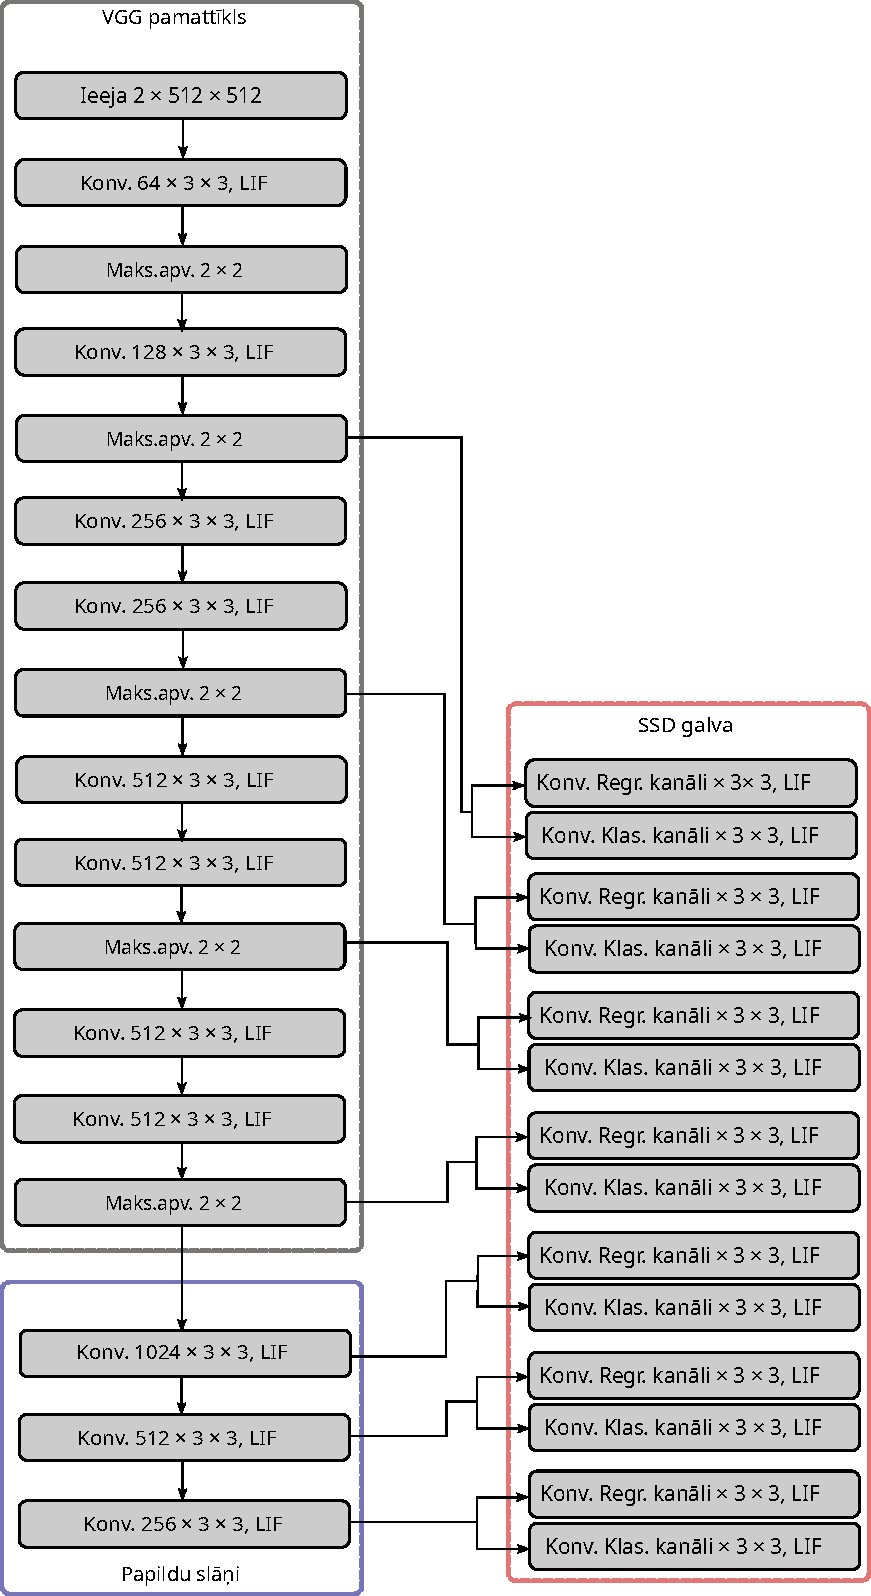
\includegraphics[width=0.5\textwidth]{fig/lv/spiking_vgg_ssd.pdf}
    \caption{Impulsu VGG pamattīkls un viena posma SSD detektēšanas galva, kas izmantoti 3D objektu detektēšanai no TVC reprezentācijām.}
    \label{fig:spiking_vgg_ssd}
\end{figure}

\begin{figure}[t]
  \centerline{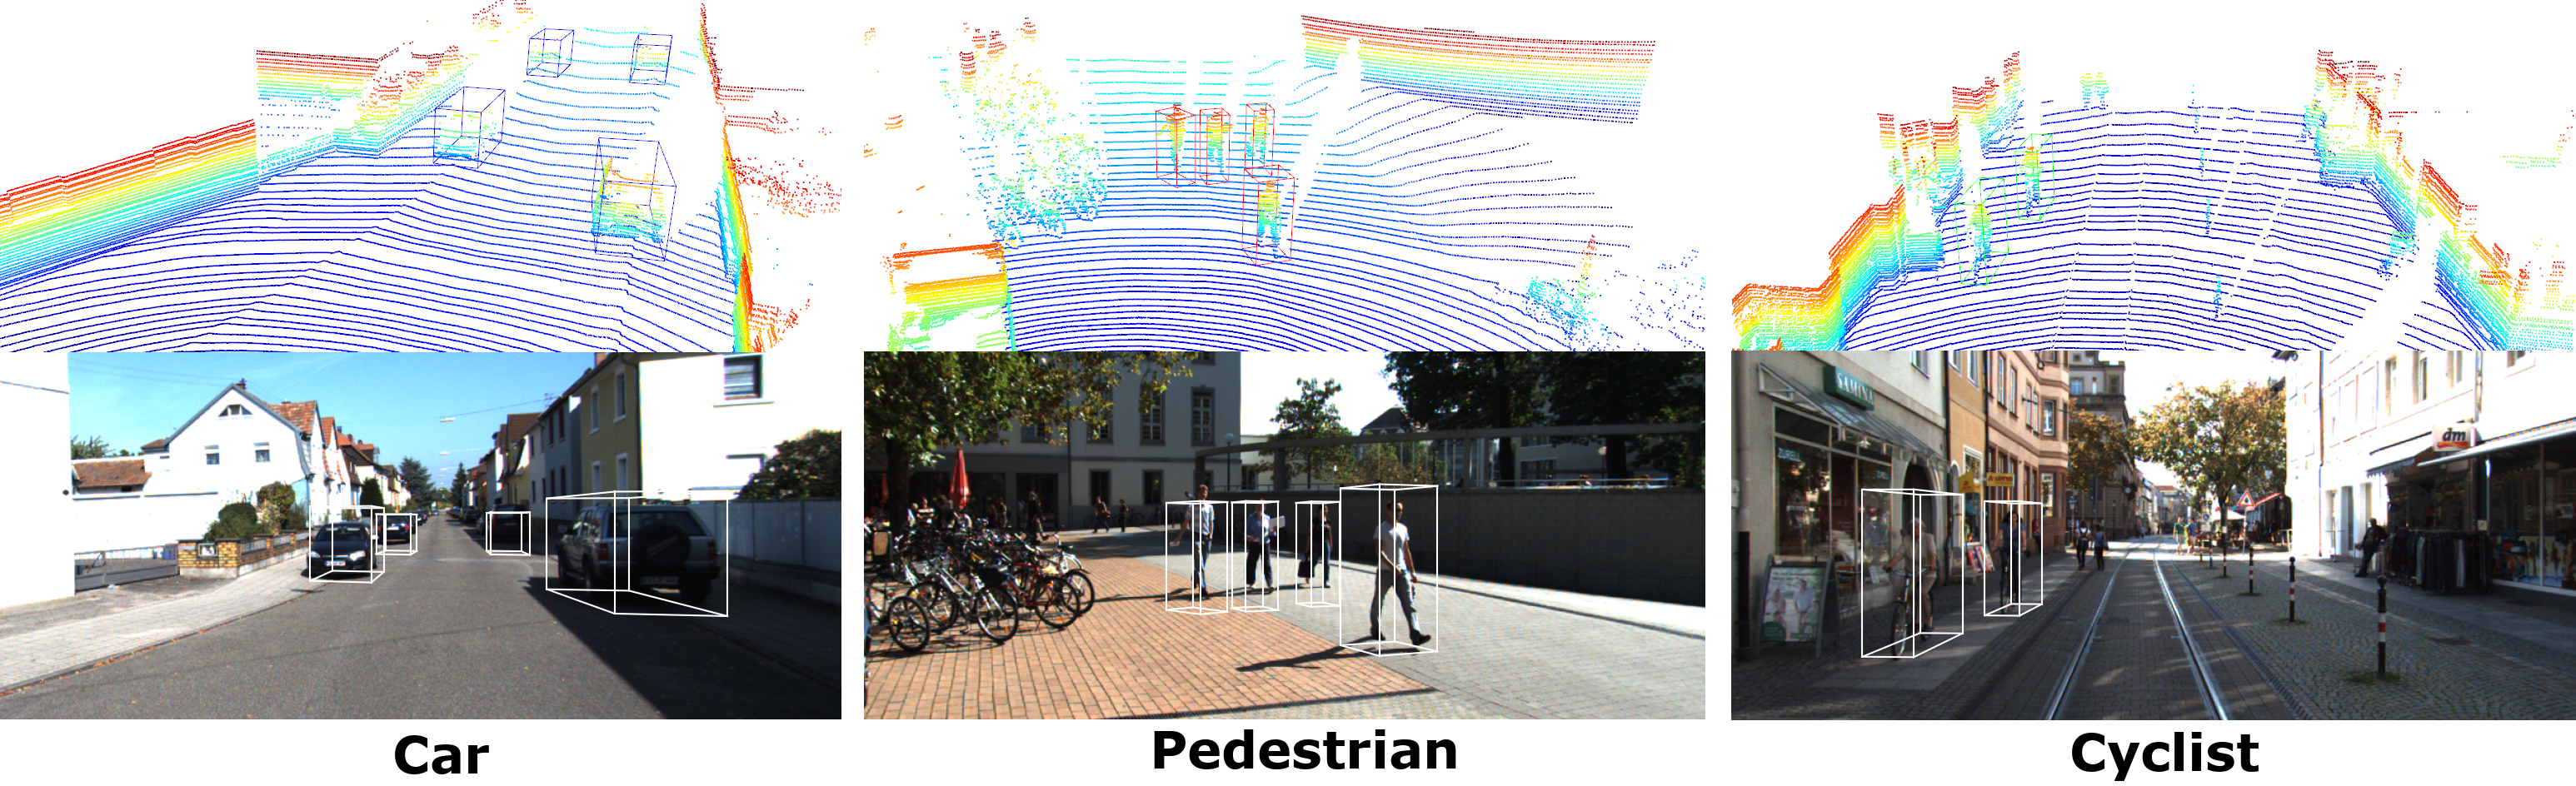
\includegraphics[width=\textwidth]{fig/7129.png}}
  \caption{3D ietverošo paralēlskaldņu detektēšanas rezultātu vizualizācija uz KITTI validācijas datu kopas attēliem.}
  \label{fig:3D_detections}
\end{figure}

Ieejas priekšapstrāde veikta, ņemot vērā ainas robežas \qtyrange{0}{50}{\metre} X asij, \qtyrange{-25}{25}{\metre} Y asij un \qtyrange{-2}{1}{\metre} Z asij, vienlaikus pētot izvēlētu vokselizācijas izmēru \([VS_x, VS_y, VS_z]\) diapazonu. Šeit \([VS_x, VS_y]\) nosaka katra \Gls{bev} šķēluma izšķirtspēju, savukārt \(VS_z\) nosaka laika soļu skaitu. \(VS_z\) iestatīts uz \qty{0.6}{\metre}, vienādi sadalot 3~m vertikālo diapazonu 5 \Gls{bev} šķēlumos un ļaujot izmantot dažādus \(t_{bin}\) izmērus, lai katrā šķēlumā iegūtu vairāk kanālu \(C\).

Abi modeļi, \textit{VGG-11} un \textit{VGG-13}, novērtēti vienādos apmācības apstākļos. Tādēļ eksperimenti ļauj analizēt vokseļu izšķirtspējas, pamattīkla dziļuma, impulsu retinājuma un parametru skaita ietekmi uz detektēšanas precizitāti.


